\documentclass[border=10pt]{standalone}

\usepackage{tikz}
\usepackage{tikzsymbols}
\usetikzlibrary{calc,patterns,shapes.geometric}

\def\centerarc[#1](#2)(#3:#4:#5){\draw[#1] ($(#2)+({#5*cos(#3)},{#5*sin(#3)})$) arc (#3:#4:#5);}

\begin{document}
	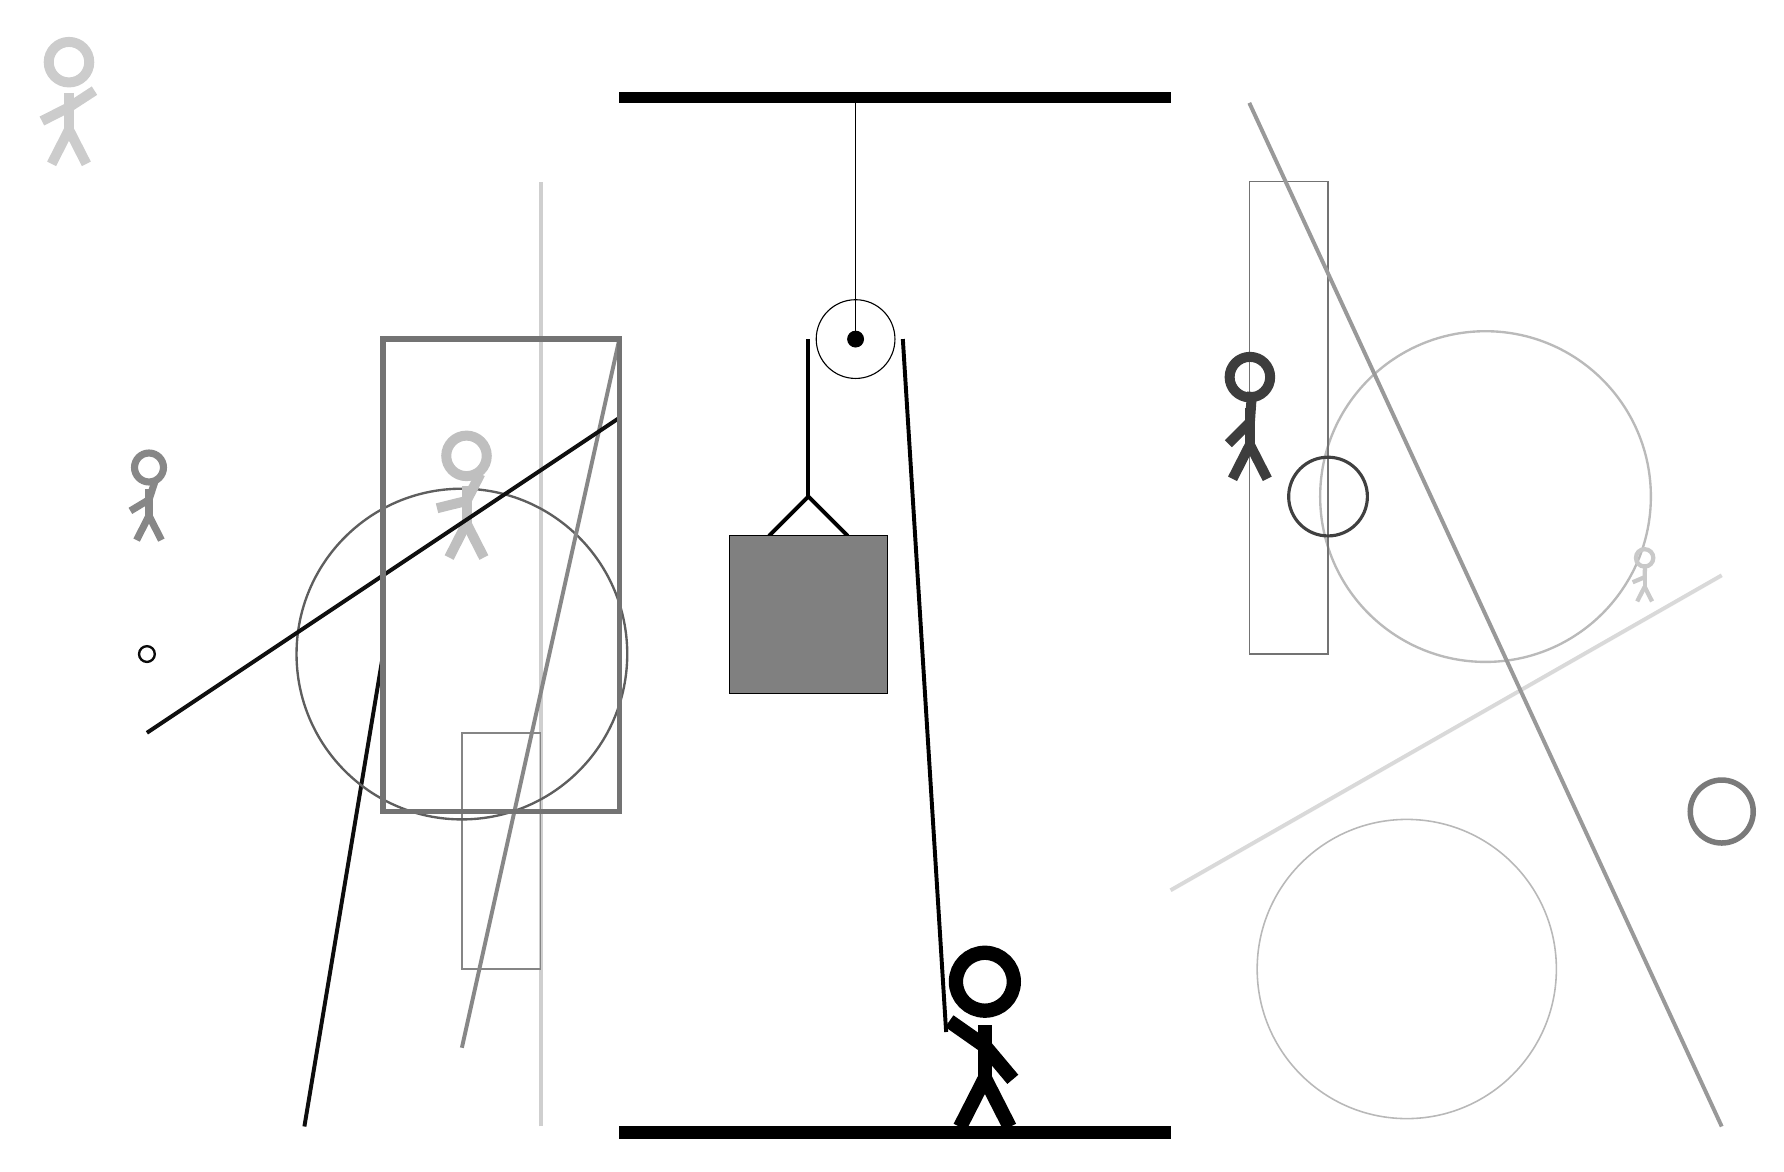
\begin{tikzpicture}
		%%%%% START %%%%%
		
		\draw[fill=black] (-2, 10) rectangle (5, 10.125);
		
		\draw (1, 7) circle (0.5);
		\draw[fill=black] (1, 7) circle (0.1);
		\draw (1, 10) -- (1, 7);
		
		\draw[line width=0.5mm] (-0.1, 4.5) -- (0.4, 5.0) -- (0.9, 4.5);
		\draw[fill=black!50] (-0.6, 4.5) rectangle (1.4, 2.5);
		
		\draw[line width=0.5mm] (0.4, 7) -- (0.4, 5.0);
		\centerarc[line width=0.5mm](1, 7)(0:180:0.6);
		\draw[line width=0.5mm](1.6, 7) -- (2.15, -1.8);
		
		\draw[line width=0.5mm, color=black!19](-3, -3) -- (-3, 9);
		
		\node[line width=0.2mm, color=black!20] at (-9, 10) {\Strichmaxerl[7][27][33]};
		\draw[line width=0.2mm, color=black!48] (-3, -1) rectangle (-4, 2);
		\node[line width=0.7mm, color=black!47] at (-8, 5) {\Strichmaxerl[5][31][72]};
		\draw[line width=0.5mm, color=black!95](-6, -3) -- (-5, 3);
		\draw [line width=0.3mm, color=black!27](9, 5) circle (2.1);
		\draw [line width=0.3mm, color=black!63](-4, 3) circle (2.1);
		
		\draw[line width=0.2mm, color=black!55] (7, 9) rectangle (6, 3);
		\node[line width=0.3mm, color=black!25] at (-4, 5) {\Strichmaxerl[7][14][63]};
		\draw [line width=0.7mm, color=black!52](12, 1) circle (0.4);
		\draw [line width=0.2mm, color=black!28](8, -1) circle (1.9);
		
		\draw [line width=0.4mm, color=black!75](7, 5) circle (0.5);
		\draw[line width=0.5mm, color=black!47](-2, 7) -- (-4, -2);
		\draw[line width=0.5mm, color=black!15](5, 0) -- (12, 4);
		\draw[line width=0.5mm, color=black!94](-2, 6) -- (-8, 2);
		\draw[line width=0.7mm, color=black!55] (-2, 7) rectangle (-5, 1);
		
		\node[line width=0.7mm, color=black!76] at (6, 6) {\Strichmaxerl[7][45][86]};
		\draw [line width=0.3mm, color=black!96](-8, 3) circle (0.1);
		\draw[line width=0.5mm, color=black!40](6, 10) -- (12, -3);
		
		\node[line width=0.3mm, color=black!21] at (11, 4) {\Strichmaxerl[3][23][88]};
		
		\node at (2.6, -1.9) {\Strichmaxerl[10][-35][-50]};
		
		\draw[fill=black] (-2, -3) rectangle (5, -3.15);
		
		%%%%% END %%%%%
	\end{tikzpicture}
\end{document}